% !TeX root = lfgw.tex
\extratitle{\LaTeX{} für Geisteswissenschaftler
\newpage

\thispagestyle{empty}
\centering{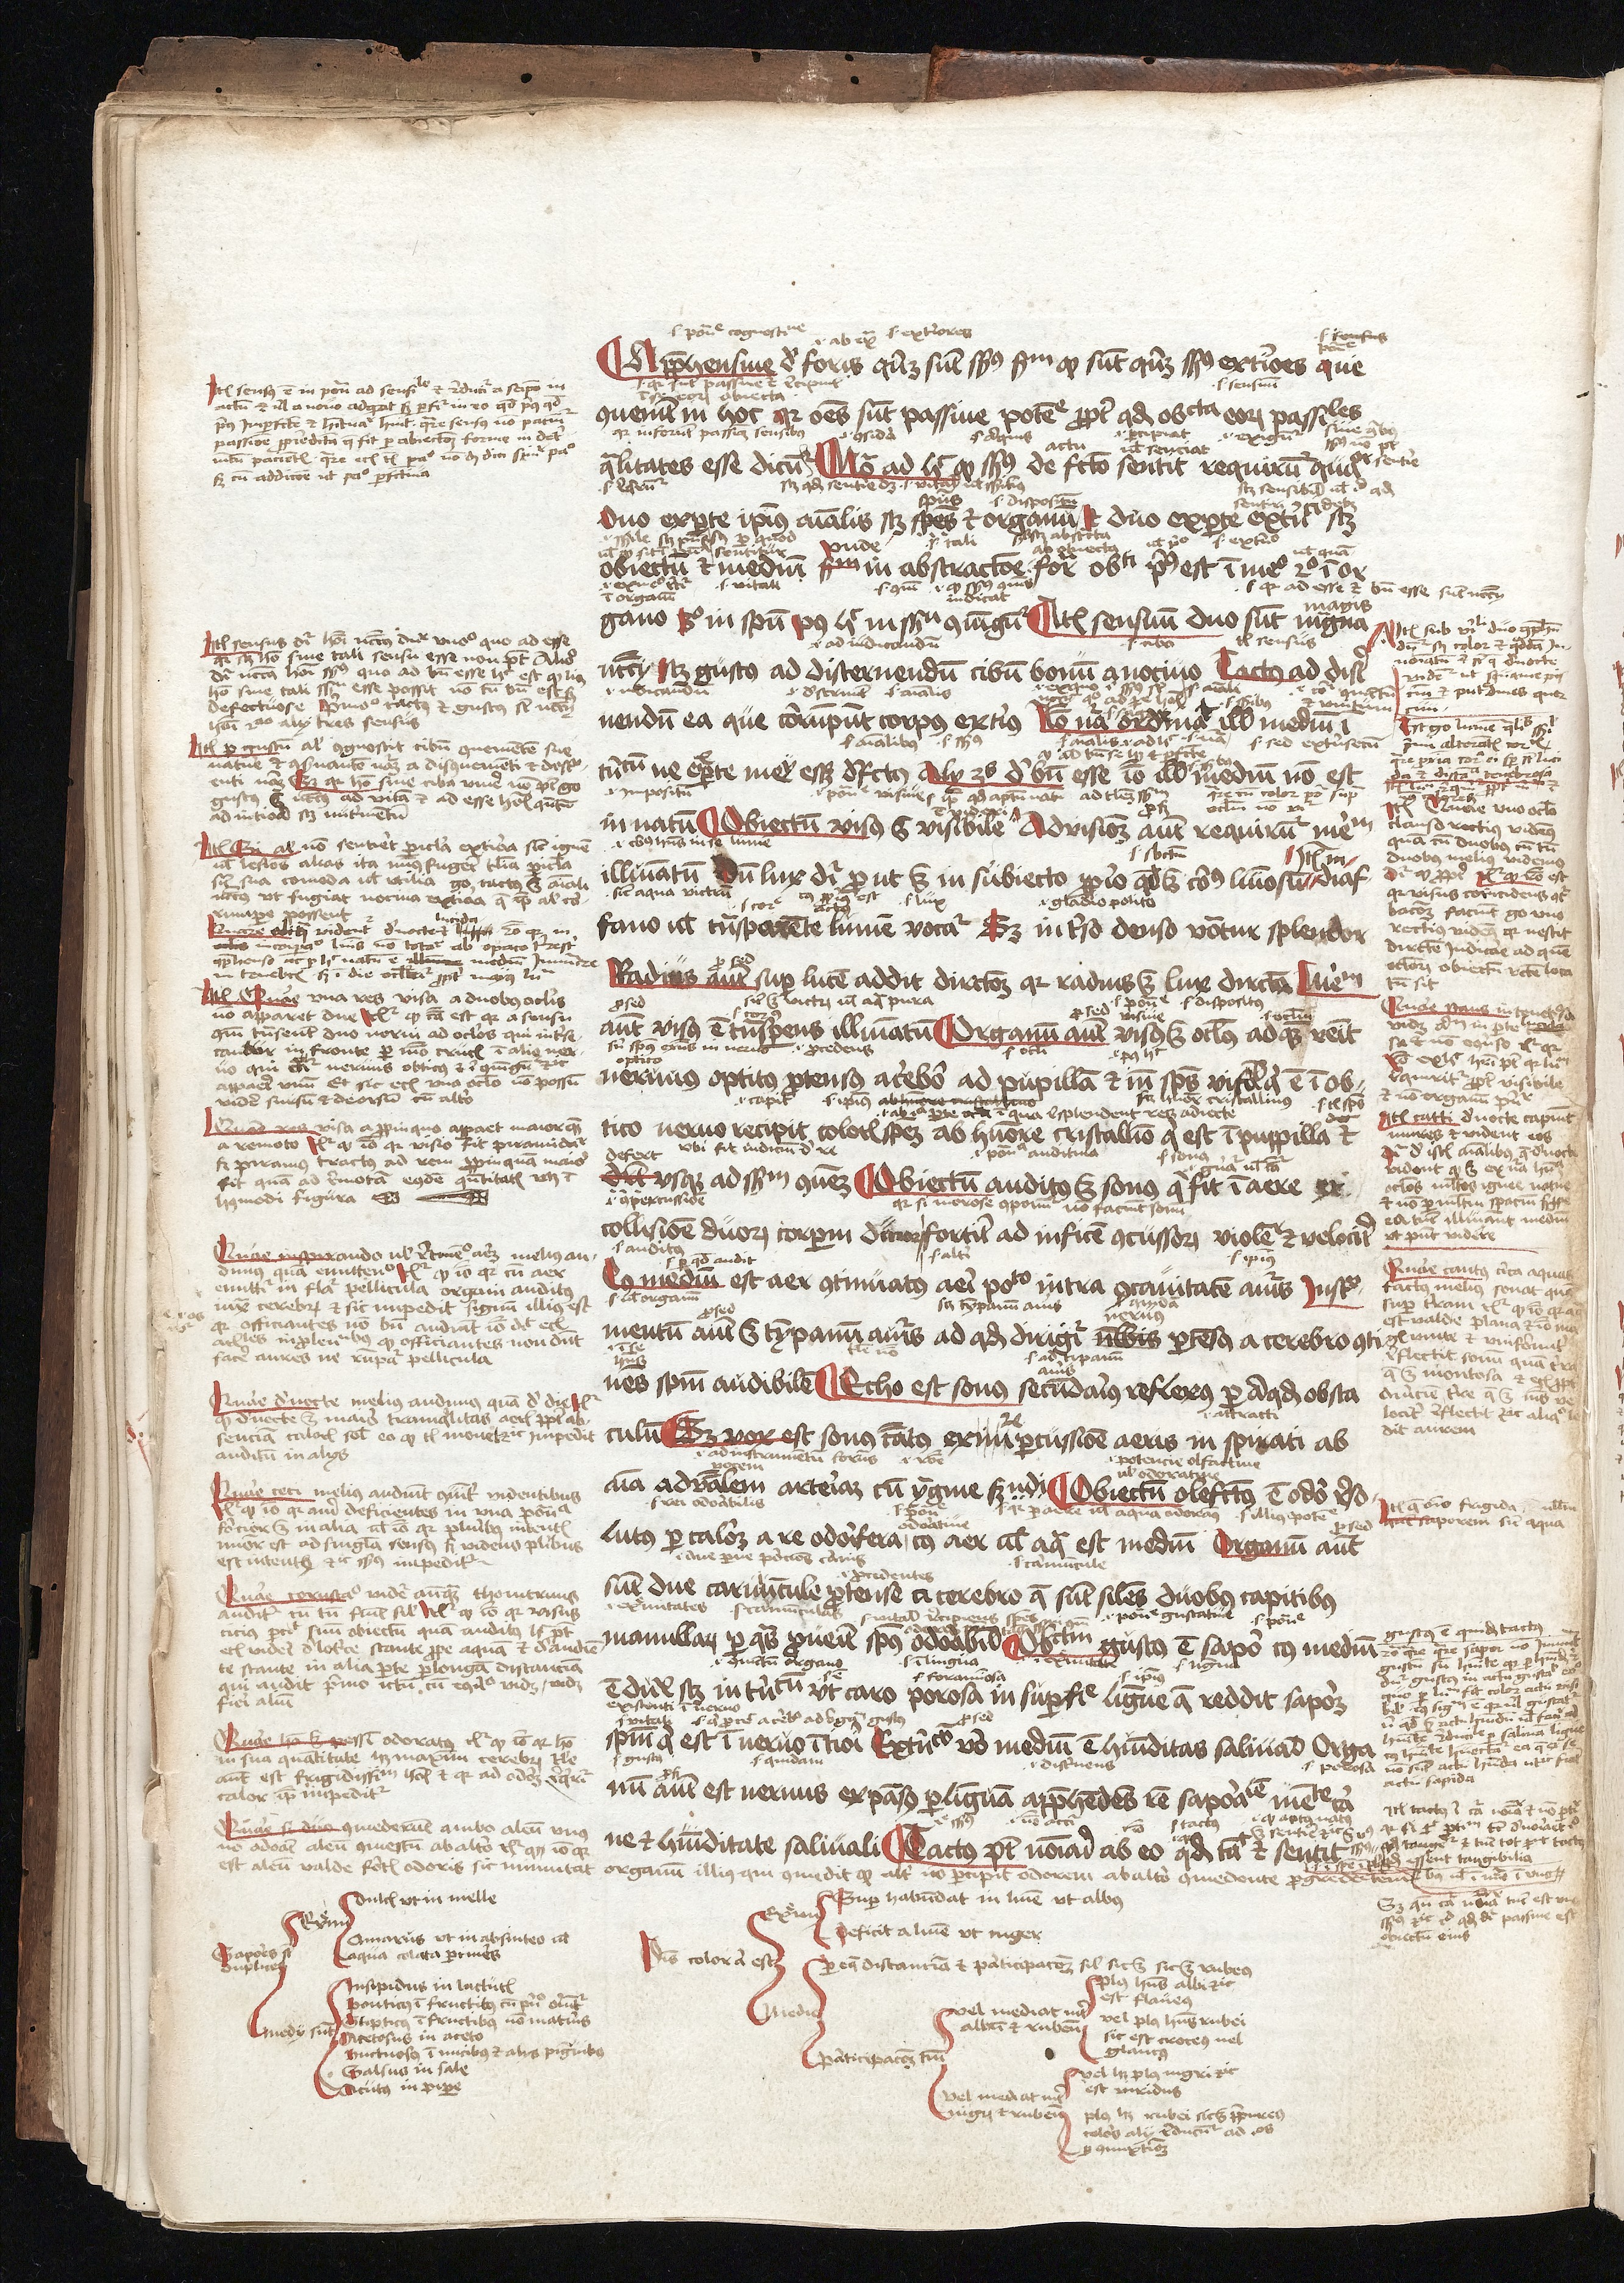
\includegraphics[width=.85\textwidth]{aristoteles_de_anima}}
\medskip

\centering{Eine Passage aus Aristoteles' De Anima in einer mittelalterlichen Handschrift mit 
Interlinear- und Marginalglossen}
}

%\subject{edition dante}

\title{\LaTeX{} für Geisteswissenschaftler}
\subtitle{Ein Überblick über die wichtigsten Hilfsmittel für die Arbeit mit 
Texten als Forschungsgegenstand}

\author{Thomas Hilarius Meyer}
\date{}
\publishers{DANTE~e.\,V.}

\lowertitleback{\copyright{} 2016 Thomas Hilarius Meyer
	Satz: thm mit \LaTeXe{} und \KOMAScript \\
        Haftungsausschluss: }

\maketitle
